\chapter{Google Architecture}
\label{chap:google_architecture}

Google is one of the well-known examples of such corporations.
Its activity directly relates to storing and processing of Big Data.
Google Search engine handles more than three billion searches every day.
Social networking service Google+ had 540 million users in 2013.
Gmail, Google's email service, had 425 million users in 2012.
These are just several examples of large-scale Google projects, that processes huge amounts of data.
Therefore, Google introduces a batch of solutions for building scalable systems. 

The overall structure of Google Big Data architecture is presented on the
Figure~\ref{fig:google_architecture}.
The lowest layer is Linux kernel, that serves as a basis for Google File System.
Google File System is a scalable and highly available file system. 
These properties are achieved by replicating data across several machines.
Next, data can be efficiently processed by MapReduce framework.
This technology includes two steps - map, that performs filtering and sorting and reduce, that aggregates the output of map step to the final result.
Bigtable, a highly scalable database, provides a way to store massive amounts of information.
Finally, client application uses these technologies to perform highly scalable and distributed tasks.  
Let us explain in more detail the primary features and internal structure of these technologies.

\begin{figure}
  \centering
  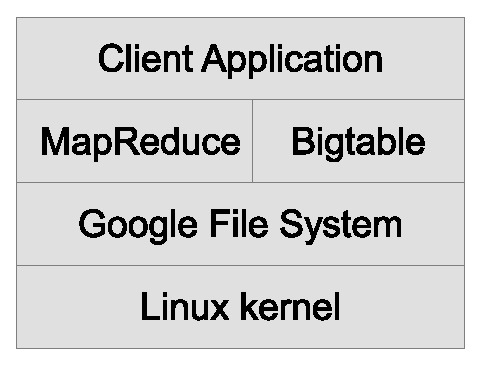
\includegraphics [width=0.9\textwidth]{images/Google_architecture}
  \caption{Google Architecture}
  \label{fig:google_architecture}
\end{figure}

\authorsection{Google File System}{SP}
[reference]
\mnote{Google File System}
Google File System (GFS) is a scalable distributed file system, which supports Big Data operations.
The underlying idea is the following: Google Search Engine and some other Google systems process vast amount of data, which is spread all over the world.
Hence the file system should be highly extensible, give an opportunity to use cheap hardware components and, consequently, be fault tolerate. 
Furthermore, it has some specific usage features.
Because of vast scales and cheap hardware, component failure is a commonplace.
The size of files exceeds several-fold the traditional standards, so a multi-gigabyte file is not unusual.
Most of the time the stored data stays unchanged and new data is only appended.
The append operation, in its turn, should provide the concurrent access for multiple clients.
GFS architecture design helps to meet all these requirements.

The Figure~\ref{fig:GFS_architecture} illustrates the main components of the GFS
Architecture.
Each GFS cluster contains one master server and several chunkservers.
The master has a "shadow" node, that provides read-only access when the primary master is down. 
Chunkserver stores chunks as Linux files on local disk.
Every chunk is replicated on several chunkservers for reliability.
One chunk combines multiple files and has a fixed size of 64 megabytes.

% Figure: according to [66]
\begin{figure}
  \centering
  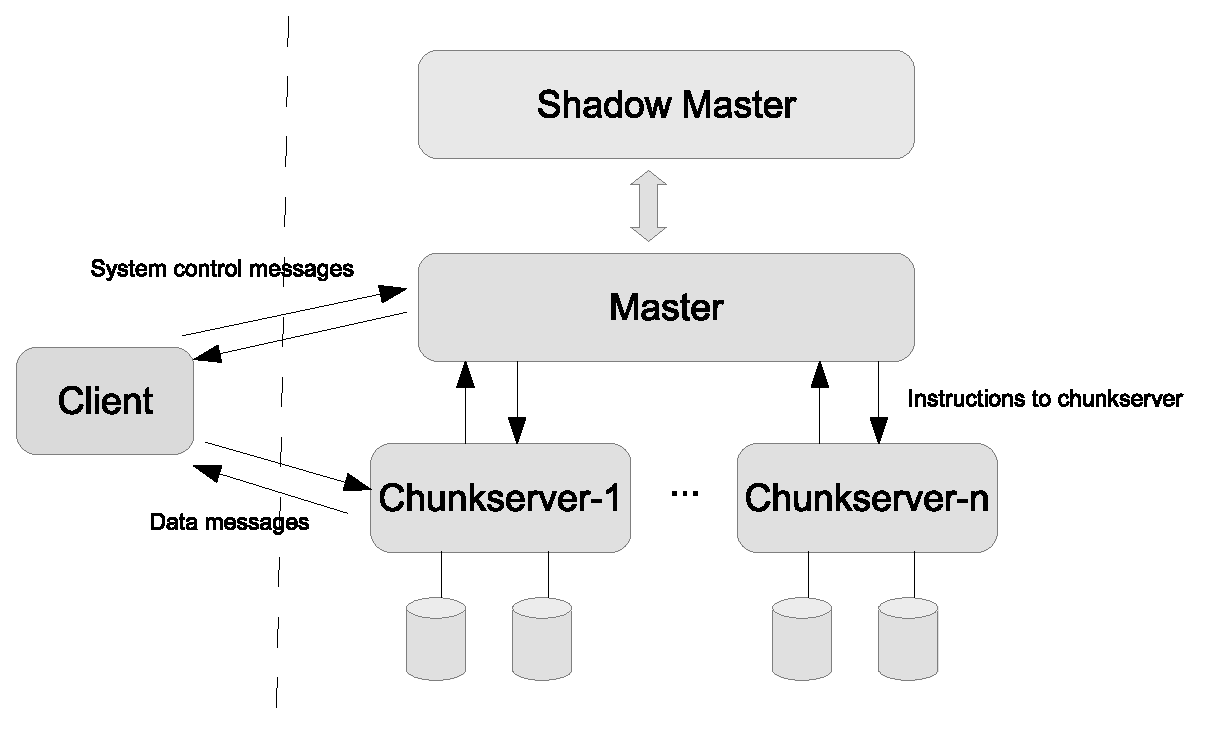
\includegraphics [width=0.9\textwidth]{images/GFS_architecture}
  \caption{GFS Architecture}
  \label{fig:GFS_architecture}
\end{figure}

The large size of chunk gives several advantages.
Clients send requests to the master for chunk location less frequently.
A persistent TCP connection to the chunkserver for a longer time period allows to avoid network overhead.
The master node stores less metadata that provide a possibility to keep it in memory.

The master node manages the mapping from files to chunks, location of chunks, access control, garbage collection and some other tasks.
It does not persistently store the information about chunks location. 
On the contrary, it gives instructions to chunkservers and collects their states using periodic HeartBeat messages.
To prevent the master being a bottleneck, only file system control data goes through it.
For example, a client can ask the master node which chunkservers it should contact.
The master node returns the corresponding chunk handle and its replicas' location.
After receiving a reply, the client caches this information and can directly transfer data to the given chunkserver, dispensing master node from overload.
Clients and chunkservers do not cache file data.
Clients mostly work with files that are too large to be cached.
Chunkservers treat chunks as Linux files, therefore in this case caching is done by operating system.

\mnote{Operation Log}
To recover its state, the master uses the operation log.
The operation log consists of the chronometric information about critical metadata changes.
This log is replicated on several machines.
For the purpose of consistency, client receives a respond for operation only when corresponding log record is flushed to a local disk and the disks of all replicas.
To avoid the operation log being too large, the master makes a checkpoint each time when the log size exceeds a certain threshold.
In the case of failure, the master can load the latest checkpoint from local disk and replay it, recovering its state.
For storing checkpoint it uses a compact B-tree like data structure, that allows to map it directly into memory and perform fast lookups.
For performance reasons the new checkpoint is created in separate thread.
The ability of a server to restore its state does not depend on the way it was terminated.
Shutting down a server by killing the process is a normal procedure. 

\mnote{Mutation}
A mutation denotes a change of the contents or metadata of a chunk.
There are two types of mutations, namely writes and record appends.
In the former case data is written with a file offset specified by a client.
In the latter, GFS chooses an offset, and data (record) is appended with an append-at-least-once semantics.
Record append operation is atomic, i.e. it is treated as one continuous sequence of bytes. 
This allows multiple clients to append information concurrently.

\mnote{Lease}
Each mutation is replicated across several chunks.
To keep a mutation order consistent at all the replicas, GFS uses a technique of leases.
The master gives a lease to one of the replicas, that becomes a primary replica.
The primary chooses an order for all the chunk's mutations and each replica then follows this order when applying mutations.

The flow of write control is shown on the Figure~\ref{fig:write_control_flow} in
more details.

\begin{figure}
  \centering
  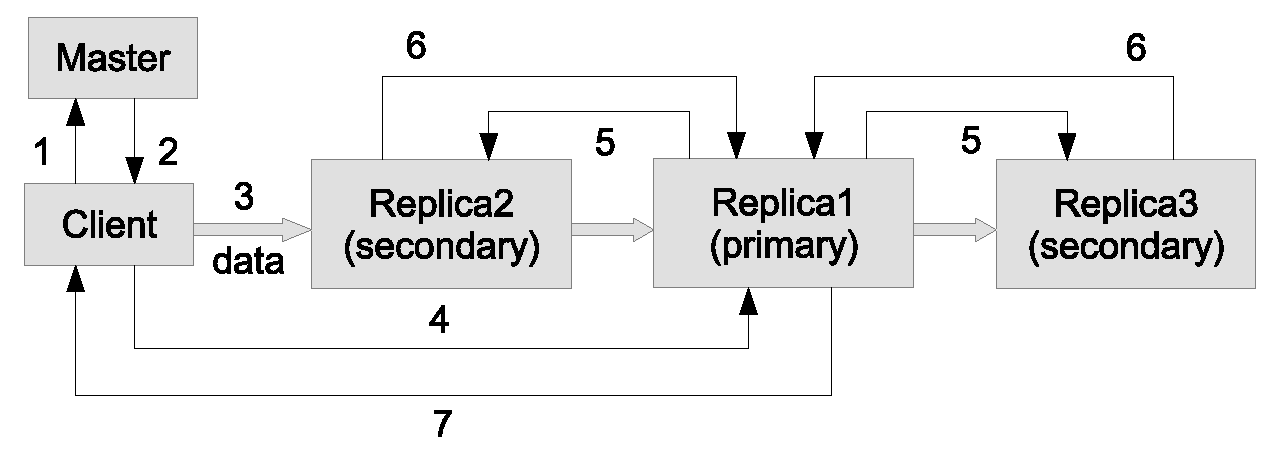
\includegraphics [width=0.9\textwidth]{images/write_control_flow}
  \caption{Write control flow}
  \label{fig:write_control_flow}
\end{figure}

1. The client sends a request to the master.

2. The master replies with a chunkserver, that holds the current lease, and the location of the other replicas.
If a primary replica (that has a lease) is not defined, the master chooses one. 
The client caches this information for the next mutations.

3. The client sends the data to all the replicas in arbitrary order.
Chunkservers store this data in an internal buffer cache. 

4. When the client receives acknowledgements from all the replicas, it sends a write request to the primary.
The primary picks serial numbers to all the mutations it has received and performs them in corresponding order.

5. All secondary replicas receive the write request forwarded by the primary.
Each replica applies mutations to its own state in the same order assigned by the primary.

6. The secondaries notify the primary about the completion of the operation.

7. The primary sends a reply to the client.
In the case of error occurrence at any of the replicas, the primary informs the client about them.
The write is considered to be successful, if the primary and an arbitrary number of secondary replicas succeeded.

GFS differs from traditional file systems in the way how it manages files and directories.
There is no possibility to list all the files in a directory in GFS, because it does not support per-directory structure.
It stores a mapping between full pathnames and metadata in a lookup table.
Prefix compression helps to efficiently represent this table in memory. 

The file deletion does not occur at once.
Firstly the master logs the event of deletion.
Than the system renames the file with a hidden name that includes the time of deletion.
The master performs a regular scan of the namespace and removes a hidden file, if it has existed for more than a specified time interval (e.g. 3 days). 

All the described features help the Google File System to successfully cope with a large-scale data processing workload.
GFS meets the storage needs of Google corporation.
Therefore Google uses GFS as the storage platform for many applications, both in research and production areas.
Another Google technologies, like MapReduce or BigTable are based on it.  	 

\authorsection{MapReduce}{SP}
[reference]
MapReduce model finds wide application in a variety of real world tasks.
For example, search engines use web crawling to gather a vast amount of information.
They process this information to create inverted indices, construct web graphs, figure out the most frequent search queries, etc.
Any of these tasks can be divided into two steps, namely Map and Reduce.
Map operation converts input data to a set of intermediate key/value pairs.
Reduce operation, in its turn, combines all the values that share the same key.
The advantage of the MapReduce abstraction is that it hides the implementation details from users.
This allows even not experienced programmers to easily construct parallel and distributed systems.

MapReduce shares the same requirements with other systems that work with large data sets.
It should provide high parallelization, be fault-tolerant and perform load balancing between nodes.
Applying Map and Reduce operations helps to parallelize large calculations.
Moreover, this makes simpler re-execution of a task that serves as a primary mechanism for fault tolerance.

Both Map and Reduce operations work with key/value pairs.
The user of MapReduce library determines the logic of these operations, specific to the given application.
The Map function receives an input a key/value pair and produces a set of intermediate pairs.
The MapReduce library groups these intermediate pairs together by the key and passes the result to the Reduce function.
It passes them via iterator that allows to handle a large data set without keeping it in memory.
The Reduce function merges the values with the same key, possibly decreasing a given set of values.
One Reduce function invocation most of the time produces a single output value, or even none.
The Figure~\ref{fig:mapreduce_pseudo_code} illustrates a pseudo-code for a simple
MapReduce task.


% instead of picture use Latex `Listinhg`
\begin{figure}
  \centering
  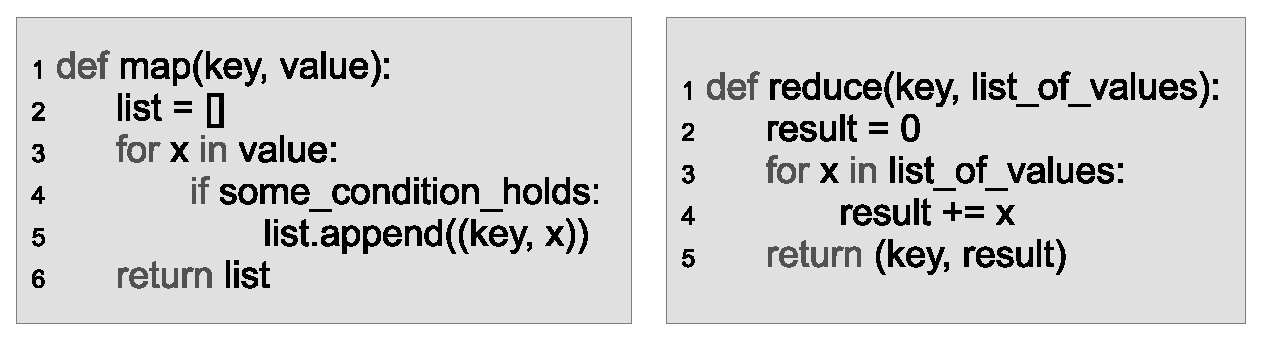
\includegraphics [width=0.9\textwidth]{images/MapReduce_pseudo_code}
  \caption{Pseudo code of the MapReduce programming model}
  \label{fig:mapreduce_pseudo_code}
\end{figure}

\begin{figure}
  \centering
  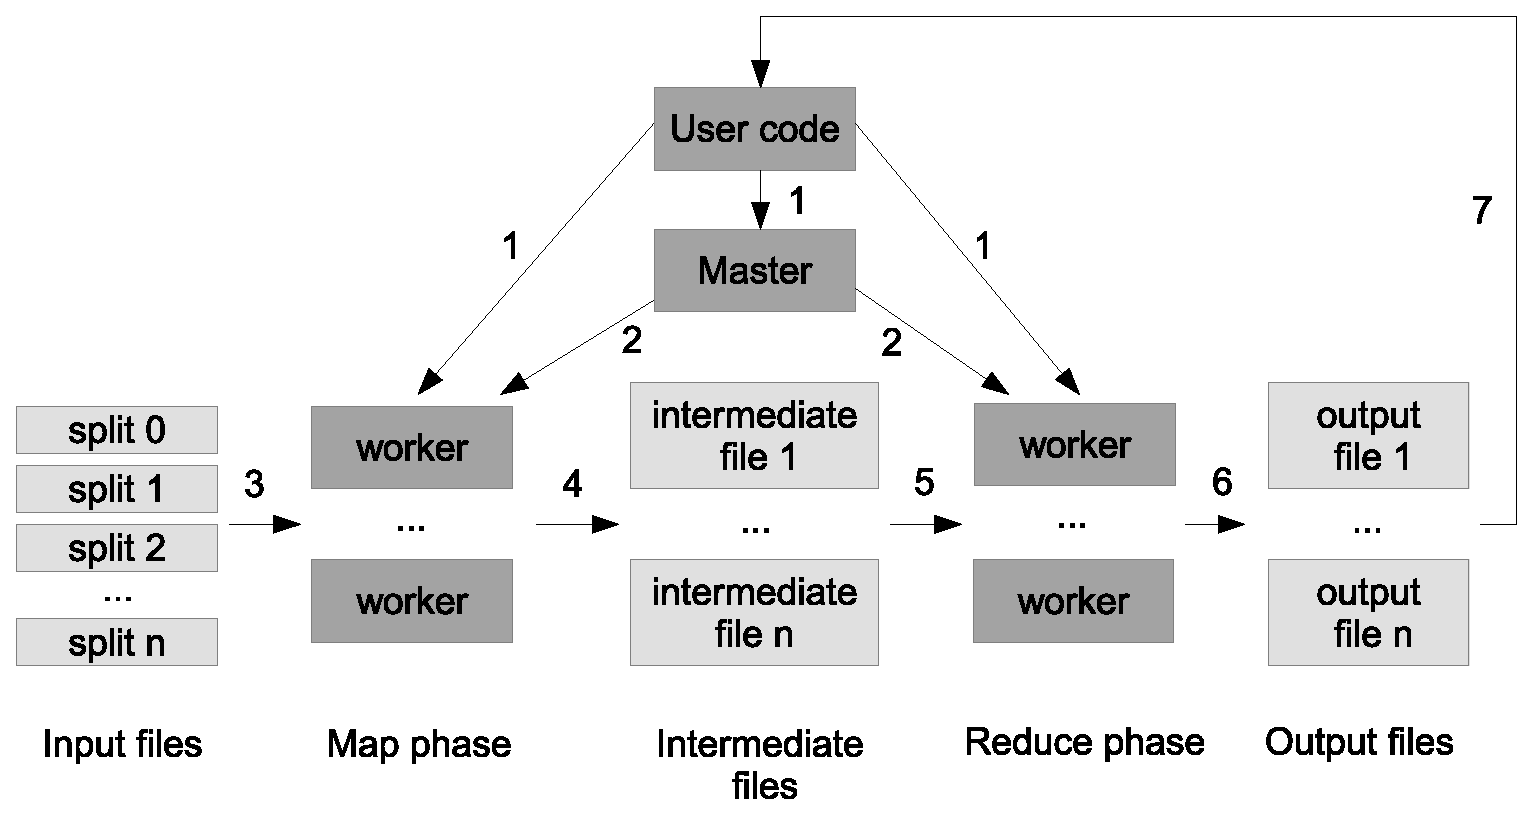
\includegraphics [width=0.9\textwidth]{images/MapReduce_operation_flow}
  \caption{MapReduce operation flow}
  \label{fig:mapreduce_operation_flow}
\end{figure}

We visualize the overall flow of a MapReduce operation in the Figure~\ref{fig:mapreduce_operation_flow}.

1. The MapReduce library divides the input files into M splits.
The size of one piece varies from 16Mb to 64Mb depending on the chosen settings.
User code invokes the MapReduce routine on several machines.

2. One of these machines is a master, while others are workers.
The master manages the workers, assigning to idle nodes one of M map tasks or one of R reduce tasks.

3. A worker that handles a map task reads the data from a respective input split.
It passes the parsed key/value pairs to the Map function.
The intermediate output of the Map function is stored in a buffer.

4. The MapReduce library periodically writes the buffered data into selected number of R local intermediate files.
Also it informs the master about the location of these files.

5. The master passes the locations to workers that handle a reduce operation.
A reduce worker reads the intermediate pairs from a specified location using remote procedure calls.
After compliting the reading, the worker groupes together all the pairs that share the same key.

6. These pairs are then passed to the Reduce function, one key and one or several related values at a time.
The output of the Reduce function is written to one of the output files.

7. After finishing all the map and reduce tasks, the MapReduce library returns the control to the user code.
The derived output files can be directly processed or be used as an input to another MapReduce task.

The MapReduce library has an optional Combine function that can be used for optimisation.
For example, let us consider the task of counting the number of words in English text.
Most probably it contains a lot of articles `a` and `the`.
Each Map task sends thousands of pairs <a, 1> to a single Reduce operation over the network. 
The Combine function can improve this situation by partial merging these pairs before sending them over the network.
Each machine that executes a Map function now also executes a Combine function.
Combine operation often uses the same code as Reduce one.
The difference is that the output of the former is stored in an intermediate file, while the latter writes it into the final output file.

The usage of Google File System (GFS) for storing input data helps to reduce the network bandwidth consumption.
GFS stores input data in blocks, copying each block on different machines (usually it makes 3 copies).
The master in MapReduce library knows which machine contains a replica and tries to assign a corresponding map task to this machine.   
When it is not possible, the master uses the nearest node to that machine.
This technology conserves network bandwidth significantly, especially when dealing with huge MapReduce operations.
 
The master keeps track of worker failures.
For this purpose it stores the state of each task and the identity of the worker that performs the task.
There are three types of states: idle, in-process and completed.
The behavior of the master in the case of failure depends on the type of the task (map or reduce) that failed.
When the map task fails, the master re-executes it on another worker.
Re-execution is required since the output of the map task is stored locally on the failed machine.
On the contrary, there is no need to re-execute the reduce task because global file system stores its output.
Sometimes a failure is caused by a defective record.
In this case the MapReduce library optionally can skip this record to continue the work. 
 
Stragglers is another problem that can obstruct the task completion.
Straggler is a machine that handles the last several map or reduce tasks too slow, keeping the whole system waiting for completion.
The MapReduce master uses a special mechanism to solve this problem.
On termination of an operation it executes the remaining in-process tasks on two different machines.
When either primary or backup worker completes computations, the task is considered to be completed.

Google Search engine widely uses MapReduce functionality for indexing, computing different statistics and analysing data.  
Moreover MapReduce can significantly facilitate the problems of data mining and machine learning.
Its key feature of dividing the computation into Map and Reduce phases helps to easily build distributed systems and makes the computation considerably more efficient.  

\authorsection{BigTable}{SP}
[reference]
Google works with large-scale data and thus it needs a distributed storage system to solve the problems of warehousing.
The company introduces its own storage system for these purposes - a Bigtable.
It is created to store petabytes of data in a distributed way.
As Google uses Bigtable in various projects, it puts different requirements on data size and latency of the storage system. 
 

% Bigtable is a distributed storage system for managing
% structured data that is designed to scale to a very large
% size: petabytes of data across thousands of commodity
% servers. Many projects at Google store data in Bigtable,
% including web indexing, Google Earth, and Google Finance.
% These applications place very different demands
% on Bigtable, both in terms of data size (from URLs to
% web pages to satellite imagery) and latency requirements
% (from backend bulk processing to real-time data serving).
% 
% A Bigtable is a sparse, distributed, persistent multidimensional
% sorted map. The map is indexed by a row
% key, column key, and a timestamp; each value in the map
% is an uninterpreted array of bytes.
% (row:string, column:string, time:int64) -> string
% 
% Every read or write of data under
% a single row key is atomic (regardless of the number of
% different columns being read or written in the row),
% 
% The row range for a table is dynamically partitioned.
% Each row range is called a tablet, which is the unit of distribution
% and load balancing
% For example, we
% store data for maps.google.com/index.html under the
% key com.google.maps/index.html. Storing pages from
% the same domain near each other makes some host and
% domain analyses more efcient.
% 
% Column keys are grouped into sets called column families,
% A column key is named using the following syntax:
% family:qualier.
% An example
% column family for the Webtable is language, which
% stores the language in which a web page was written. We
% use only one column key in the language family, and it
% stores each web page's language ID. Another useful column
% family for this table is anchor; each column key in
% this family represents a single anchor, as shown in Figure
% 1. The qualier is the name of the referring site; the
% cell contents is the link text.

% Each cell in a Bigtable can contain multiple versions of
% the same data; these versions are indexed by timestamp.
% Bigtable timestamps are 64-bit integers. They can be assigned
% by Bigtable, in which case they represent real time in
% microseconds, or be explicitly assigned by client applications.
% To make the management of versioned data less onerous,
% we support two per-column-family settings that tell
% Bigtable to garbage-collect cell versions automatically.
% The client can specify either that only the last n versions
% of a cell be kept, or that only new-enough versions be
% kept (e.g., only keep values that were written in the last
% seven days)